\documentclass[a4j,10pt]{jsarticle}
\usepackage{layout,url,resume}
\usepackage[dvipdfmx]{graphicx}
\usepackage{setspace}
\pagestyle{plain}
\setstretch{0.62}
\begin{document}
%\layout

\title{骨格推定を用いたボディビルのポージング練習ツールの提案}

% 和文著者名
\author{
    otot(田崎和輝)\thanks{NECO}
    \and
    親:ks91(斉藤賢爾) \thanks{NECO}
}

% 和文概要
\begin{abstract}
ボディビル大会に出場するためにはトレーニング、減量とともにポージングの練習も大切である。しかしながら、初心者が1人で練習するには難しく、トレーナーなどから指導を受けることもできるが高価である。
今回はこのような課題を解決するために、骨格推定技術を利用し、練習中にリアルタイムでフィードバックを行うことで初心者単身でもポージング練習ができるシステムを作成し、その有効性について8人の被験者に対し実験を行った。

\end{abstract}

\maketitle

\section{はじめに}
ボディビルをはじめとするフィットネス大会に出場する人は増加傾向にある。日本ボディビル・フィットネス連盟(JBBF)の登録選手数は2015年の2213人から2021年の5576人へと2倍位以上に増加している\cite{jbbf}。
しかしながら、ボディビル大会への出場は敷居が高く、トレーニング、減量だけでなくステージでの見栄えを良くするためにポージング練習も必須となる。
ポージング練習は初心者一人で行うのは難しく、トレーナーに指導を受けるという方法があるが高額である。
本研究では、骨格推定ライブラリであるOpenPoseを用いてカメラの入力から理想のポーズとの関節角度を比較し、視覚的にフィードバックを返すシステムを構築した。
\section{背景}
ボディビルとは、筋肉の発達度、そのダイナミックさ、美しさ、またバランスなどを競い合う個人スポーツである。\cite{bodybuilding}
ボディビルでは審査で規定の7ポーズをとる。審査基準は筋肉の大きさ、形と明白さ、鮮明さ、バランス、ポーズの流れ、表現法などによる。\\
\indent
骨格推定とは深層学習などを用いて人物のポーズを可視化してくれる手法であり、モーションキャプチャーなどの機器を使用することなく,
画像、動画データ、又はカメラからの入力を用いて人間のポーズを可視化することができる。
カーネギーメロン大学(CMU)の Zhe Caoら が「Realtime Multi-Person pose estimation」\cite{openpose}の論文で発表した、OpenPoseが一つの例である。
\subsection{関連研究}
武蔵野大学の鎌田らは \cite{Relatedresearch1}スクワットのフォームに対してOpenPoseを用いて姿勢差分に用いる関節角度の抽出方法とについて実装した。
また、広島市立大学の岡本らは \cite{Relatedresearch2}陸上のハードル跨ぎの練習においてKinectを用いて骨格を推定し、リアルタイムでフィードバックを返すシステムを提案した。


%---------------------------------------------

\section{問題}
既存の鏡の前で自分を見ながら行う練習方法では理想との差異が分かりにくい。鏡の前で行うポージング練習では1人ではポーズを改善することが難しい

\section{仮説}
理想のフォームとの差異をリアルタイムにフィードバックを行いながらポージング練習を行うことで初心者でも1人で理想のフォームに近づくことができると考えた。


\section{設計}
理想のポーズとする画像からOpenPoseで各関節座標を計測し、関節角度を計測する。ユーザーはカメラに向かいポージングを行う。ユーザーの座標から関節角度を計測し、理想のポーズの関節角度に対して角度が正負両方の方向に対して5度以上異なる場合はその角度を修正するために動かす骨を赤く表示する。角度が正しい場合は緑で表示する。
\section{実験}
\subsection{実験概要}
理想のポーズと練習後のユーザーのポーズの関節角度を比較しその差を評価した。
鏡を見て練習を行った群(A群)と今回のシステムを使い練習をした群(B群)を比較し、今回のシステムが与える影響を検証した。
\subsection{実験方法}
今回はボディビルのポージングの中で大きな役割を果たす肩関節、肘関節に注目し角度を取得する。理想とするポーズはJBBF公式YouTubeの「JBBF BODYBUILDING ポージングレッスン」\cite{aizawa}
の動画の2022 第68回 日本男子ボディビル選手権大会男子ボディビル優勝者の相澤隼人選手のフロントダブルバイセップスポーズとした。
被験者に対し、フロントダブルバイセップスを10秒、休憩を10秒を1セットとし10セット練習を行わせ、終了後、鏡やフィードバックなしでポーズを計測した。
\subsection{実験結果}
各群の練習前後の理想のフォームの角度の差の平均は(表1)のようになった。
鏡を見て練習を行った群(A群)と今回のシステムを使い練習をした群(B群)ともに理想のフォームとの差が大幅に小さくなることはなかった。
\begin{center}
    \begin{tabular}{|l|r|r|} \hline
      \multicolumn{3}{|c|}{各群の練習前後の理想のフォームの角度の差の平均} \\ \hline
      群 & 練習前(度) & 練習後(度) \\ \hline
      A群 & 8.7 & 7.95 \\
      B群& 7.65 & 8.1 \\ \hline
    \end{tabular}
\end{center}
(表1)\\
練習前後の関節角度の左右差に着目すると、A群では肩関節は4人のうち悪化した者が1名、変化が無かった者が2名、改善されたものが1名だったのに対し、
B群では悪化した者が改善された者が2名,変化がなかった者は1名、改善された者が2名だった。図\ref{elbow} \\
肘関節に関してはA群では4人のうち悪化した者が0名、変化が無かった者が1名、改善されたものが3名だったのに対し、
4人のうち悪化した者が1名、変化が無かった者が0名、改善されたものが3名だった。 図\ref{shoulder}
\begin{figure}[htbp]
    \begin{center}
        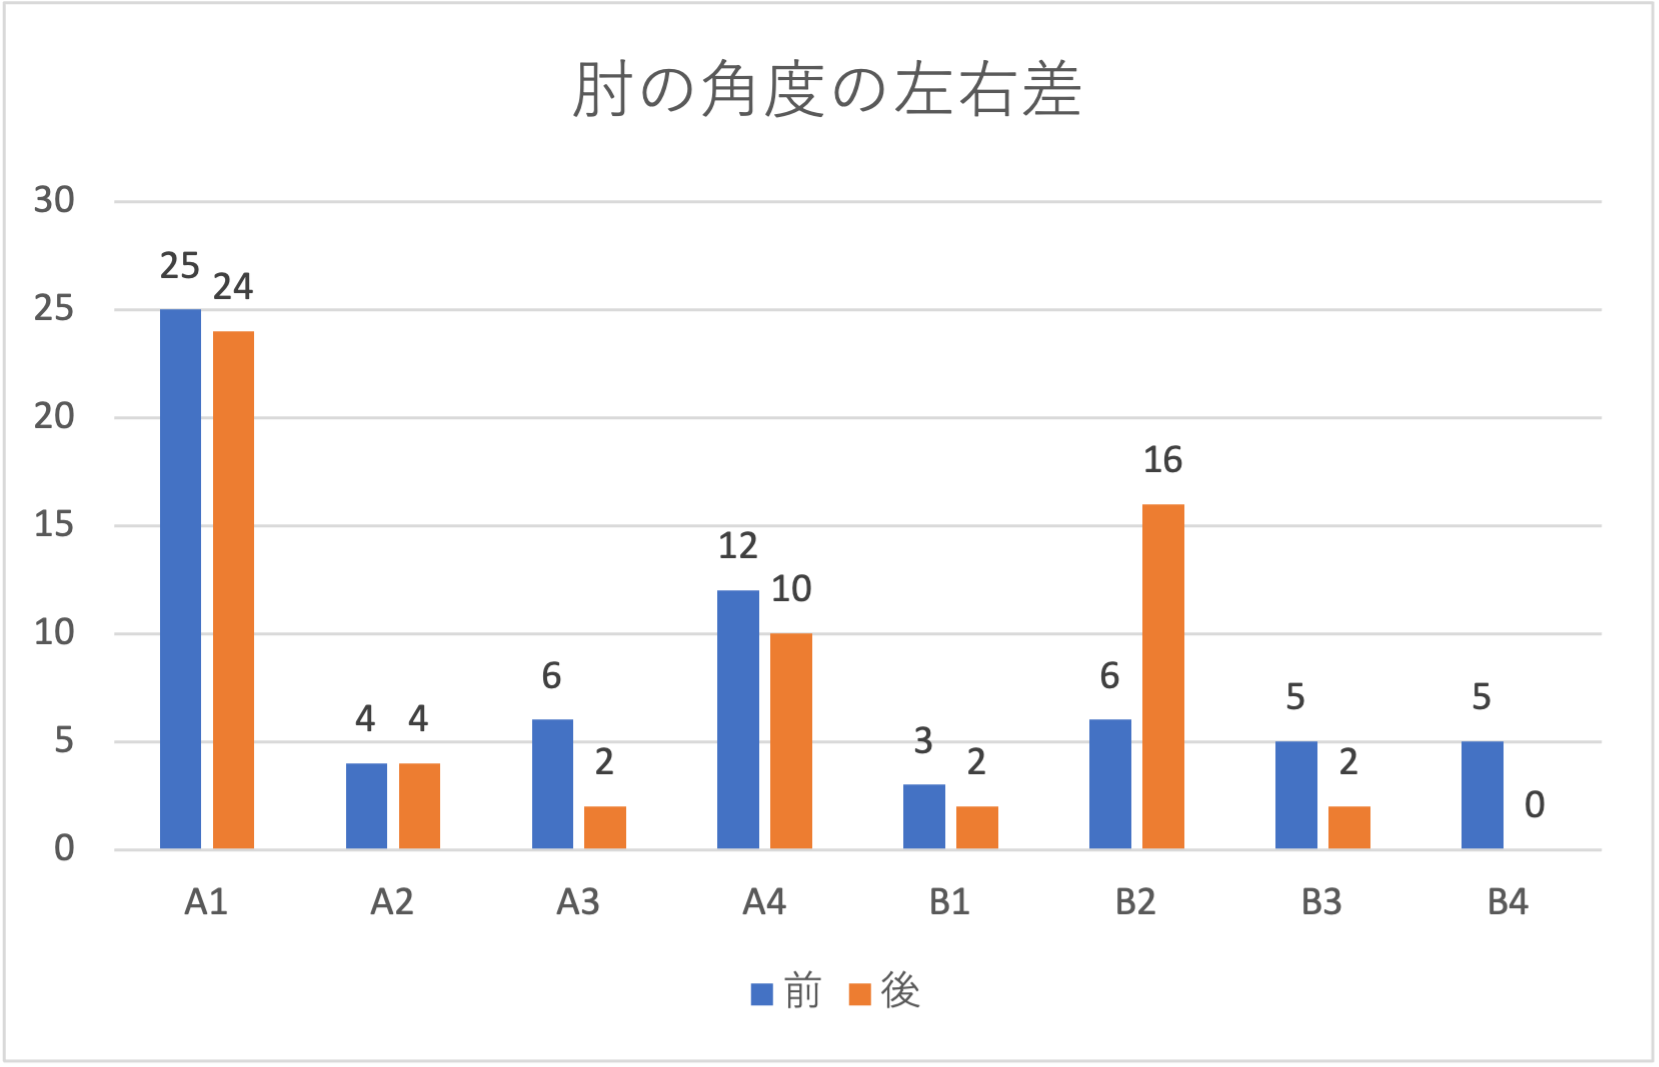
\includegraphics[width=6cm]{elbow.png}
        \caption{肘の角度の左右差}
        \label{elbow}
    \end{center}
\end{figure}
\begin{figure}[htbp]
    \begin{center}
        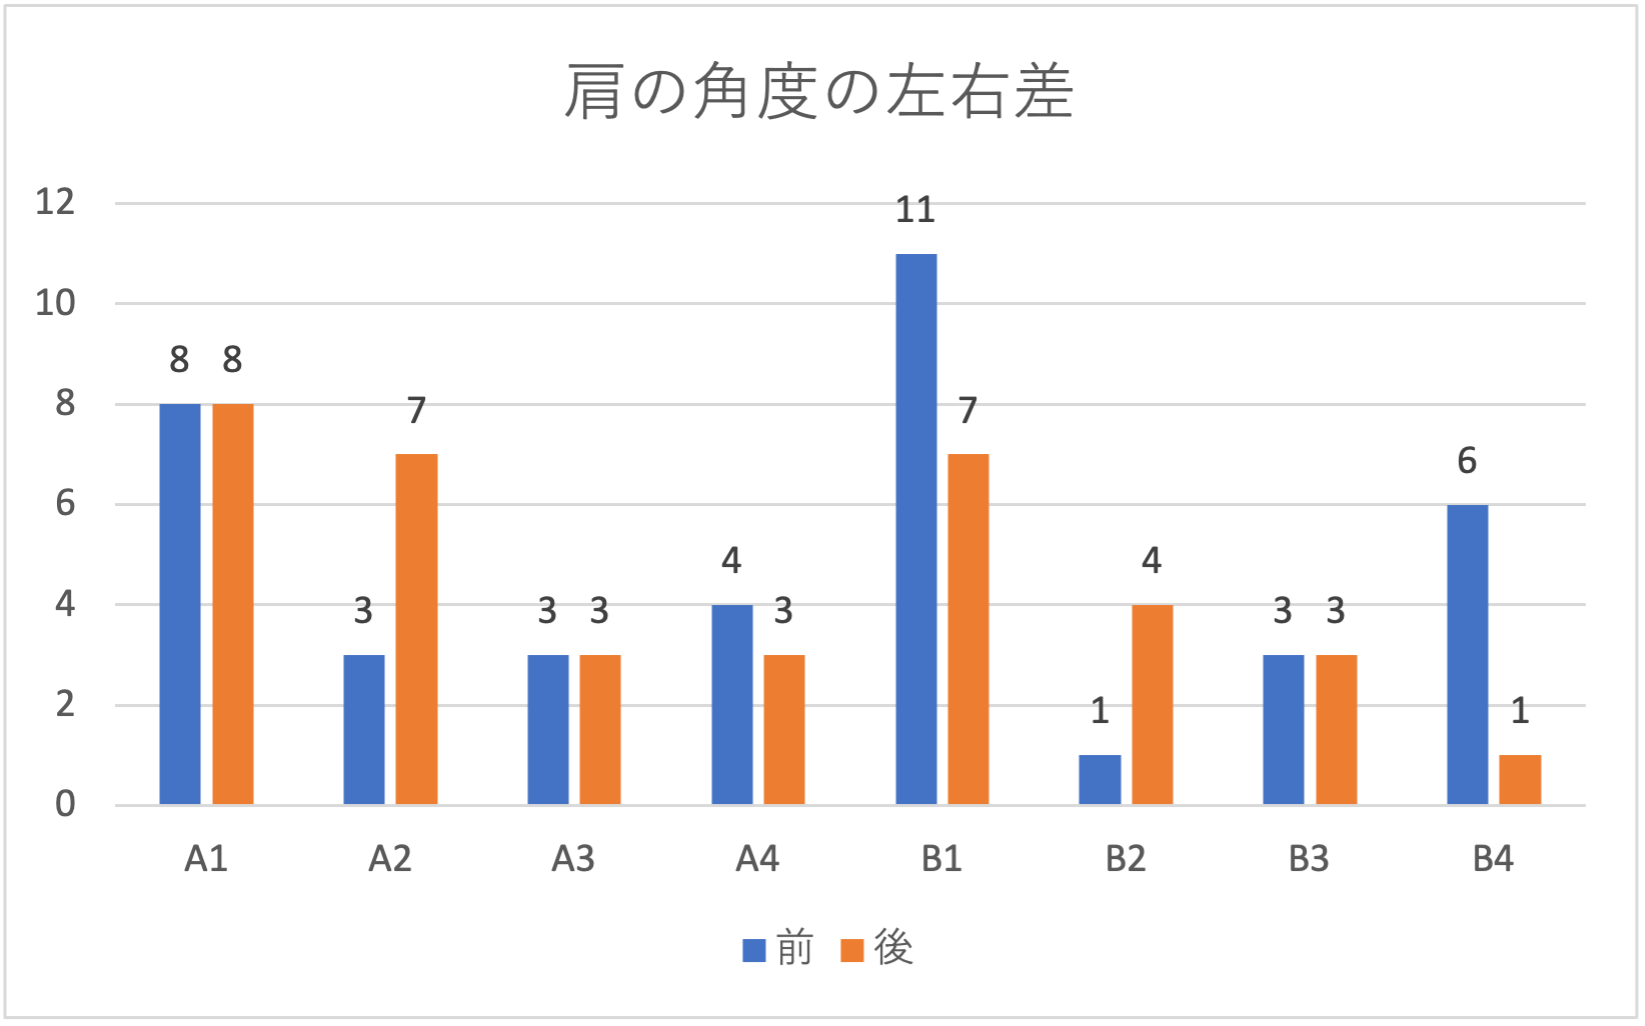
\includegraphics[width=6cm]{shoulder.png}
        \caption{肩の角度の左右差}
        \label{shoulder}
    \end{center}
\end{figure}
\section{考察}
今回の実験ではこのシステムでは既存の鏡の前で行うポージング練習と大きな差が出ることはなかった。原因として考えられることは2点ある。
\begin{enumerate}
    \item フレームレートが低かったためスムーズにフィードバックを与えることができなかった。
    \item フィードバックの与え方に問題があった。
\end{enumerate}
1に関しては、今回の環境では0.5~0.8fpsほどでしか動作しなかった。そのため、
被験者がフィードバックをうまく受けることができなかったと推測される。\\
2に関しては、今回は理想の角度から開きすぎているのか、閉じすぎているのかを確認することができず指定の範囲に近づくのに時間がかかってしまったと考えられる。\\
一方で、関節角度の左右差というところで見ると今回のシステムを利用して改善されている可能性がある。練習後悪化した被験者も1名いたが、この被験者は練習前の時点で全被験者の中で理想のフォームに一番近かった被験者であり、
上で述べたシステムがうまく作用しなかった原因と考えられるものによって悪影響が出てしまったとも考えられる。
\section{おわりに}
骨格推定を用いたリアルタイムでフィードバックをするボディビルのポージング練習の有効性を検証するために、8人の被験者に対して実験を行った。
今回の実験では既存の鏡を用いたポージング練習に対して有効であるという結果は検証できなかった。しかしながら、システムを利用することでユーザーの左右差を小さくすることができる可能性が示された。
システムの改善、仮説の再検討を行っていけば、ボディビルダーにとって有効なシステムを作ることができると考えられる。

\bibliographystyle{junsrt}
\bibliography{resume}

\end{document}
% end of file
